% Перестроение поверхности в 3d.
\subsection{Методы перестроения поверхности в трехмерном случае}

\subsubsection{Архитектура неструктурированной поверхностной расчетной сетки}

Решение задачи перестроения поверхности будем рассматривать на неструктурированной поверхностной расчетной сетке с треугольными ячейками.
Элементами расчетной сетки являются узлы ($N$), ребра ($e$) и треугольные ячейки ($f$).
Для удобства каждый элемент сетки связан со всеми своими инцидентными элементами: так связаны между собой инцидентные узлы и ребра, узлы и ячейки, ребра и ячейки (см. рис.~\ref{fig:text_1_remesh3_architecture}).
Множество инцидентных узлов рассматриваемого ребра или ячейки будем обозначать $\mathscr{N}$, множество инцидентных ребер рассматриваемого узла или ячейки будем обозначать $\mathscr{E}$, множество инцидентных ячеек рассматриваемого узла или ребра будем обозначать $\mathscr{F}$.

\begin{figure}[ht]
\centering
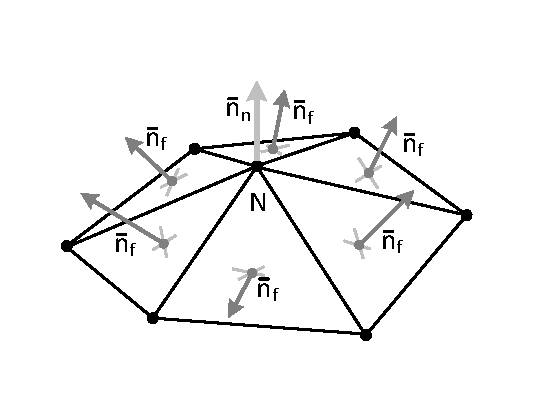
\includegraphics[width=0.5\textwidth]{pics/text_1_remesh_3d/pic_architecture.pdf}
\captionstyle{center}\caption{Архитектура расчетной сетки.}
\label{fig:text_1_remesh3_architecture}
\end{figure}

К расчетной сетке предъявляются следующие требования.
Во-первых, сетка должна быть целостной, то есть каждое ребро имеет ровно два инцидентных узла, отсутствуют изолированные и висячие узлы, а также изолированные ребра.
Во-вторых, все ячейки должны представлять собой треугольники (это гарантирует, что ячейка является плоской, так как четыре и более произвольных узлов могут не лежать в одной плоскости).
И в-третьих, рассматриваются только замкнутые сетки, представляющие собой поверхности, то есть каждое ребро имеет ровно две инцидентные ячейки (отсутствуют граничные ребра).
\begin{equation}\label{eqn:text_1_remesh3_arch}
\begin{cases}
\forall N \implies \mathscr{E}(N) > 2, \mathscr{F}(N) > 2, \\
\forall e \implies \mathscr{N}(e) = 2 , \mathscr{F}(e) = 2, \\
\forall f \implies \mathscr{N}(f) = 3 , \mathscr{E}(f) = 3. \\
\end{cases}
\end{equation}

\

В качестве дополнения также будем требовать, чтобы сетка представляла собой двустороннюю поверхность, для каждой ячейки однозначно определена нормаль к поверхности $\overline{n}_f$.
Также никакие два узла сетки не совпадают и отсутствуют ячейки с нулевой площадью (так как это сделает невозможным вычислений нормалей).
Для узла сетки будем рассматривать понятие нормали к поверхности и определять эту нормаль как
\begin{equation}
\overline{n}_n(N) = \frac{1}{|\mathscr{F}(N)|} \sum_{f \in \mathscr{F}(N)}{\vec{n}_f(f)}.
\end{equation}

%---------------------------------------------------------------------------------------------------

\subsubsection{Классические методы перестроения поверхности}

Центральная задача перестроения поверхности из-за накопления льда внутри ячеек расчетной сетки выглядит следующим образом.
Пусть известно, что в результате численного решения задачи ледообразования конечно-объемным методом \cite{Beaugendre2003Ice} в каждой ячейке сетки была вычислена масса накопленного льда ($m$).
Будем считать плотность льда постоянной, то есть в каждой ячейке также известен объем накопленного льда ($V$).
Для каждого узла сетки $N$ требуется найти его новое положение в пространстве $N'$, чтобы для каждой ячейки с узлами $ABC$ объем пространства, ограниченный фигурой $ABCA'B'C'$ соответствовал объему льда, накопленному в данной ячейке.

Следует отметить, что поставленная задача может не иметь точного решения, и в этом случае следует стремиться к минимизации ошибки по объему (когда фактически образовавшийся объем льда не слишком сильно отличается от целевого объема, то есть разница $V_{ABCA'B'C'} - V$ мала).

Задачу определения новых положений узлов расчетной сетки можно разделить на две задачи: определение направлений смещения узлов и определение величин смещения.

Простейшие классические методы перестроения выполняются в предположении, что направление смещения узла совпадает с нормалью, проведенной из этого узла.
Таким образом, необходимо лишь определить величину смещения.

\begin{figure}[ht]
\centering
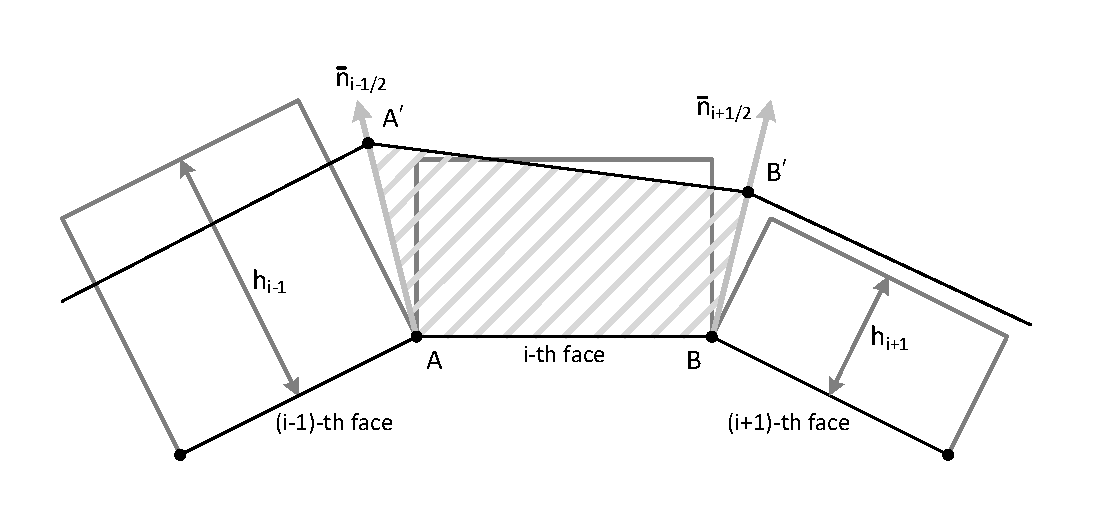
\includegraphics[width=\textwidth]{pics/text_1_remesh_3d/pic_classical_methods_rectangles.pdf}
\caption{Rebuilding the surface using the method of rectangles in 2D.}\label{fig:pic_classical_methods_rectangles}
\end{figure}

\begin{figure}[ht]
\centering
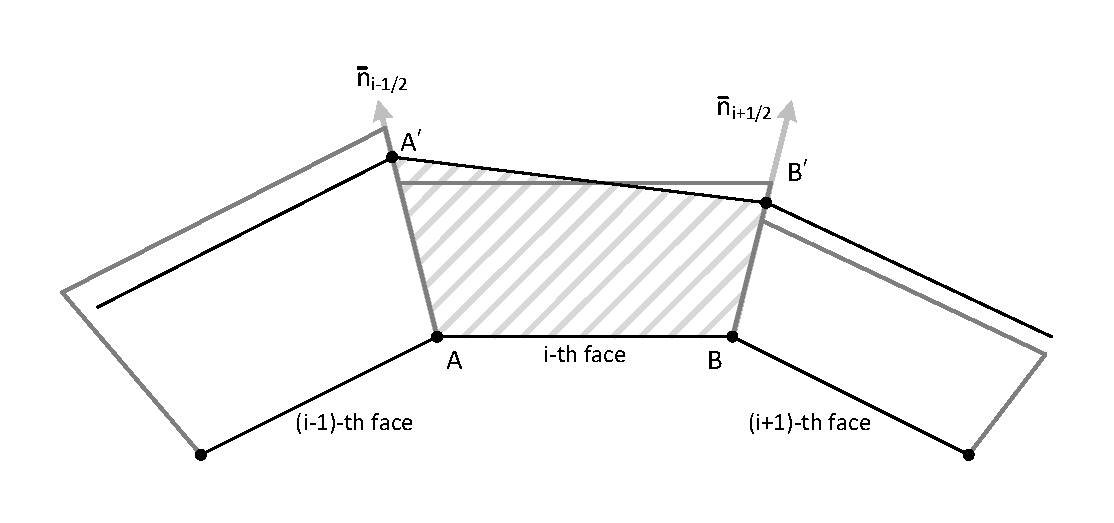
\includegraphics[width=\textwidth]{pics/text_1_remesh_3d/pic_classical_methods_trapezoids.pdf}
\caption{Surface rebuilding using the trapezoids method in 2D.}\label{fig:pic_classical_methods_trapezoids}
\end{figure}

As the first method, let's consider the prisms method (in the two-dimensional setting, this method is analogous to the method of rectangles, shown in Fig.~\ref{fig:pic_classical_methods_rectangles}).
In this method, the input data is the amount of accumulated ice in each mesh face ($V(f)$).
At the first step, the thickness of the ice cover is searched for in each face, assuming that the ice within one face has the shape of a prism, and the face is the base of this prism.
Then, the thickness of the ice cover is equal to $h(f) =
\frac{V(f)}{S(f)}$, where $S(f)$ is the face area.
After that, the displacement value of each node is calculated simply
as the arithmetic average of the ice cover heights in all incident
faces
\begin{equation*}
h(N) = \frac{1}{|\mathscr{F}(N)|} \sum_{f \in \mathscr{F}(N)}{h(f)}.
\end{equation*}

The second method can be called the pyramids method (in a two-dimensional setting, this method is analogous to the trapezoids method shown in Fig.~\ref{fig:pic_classical_methods_trapezoids}).
The input data is also the volume of accumulated ice in each mesh face ($V(f)$).
However, unlike the previous method, the volume of ice accumulated in the face is represented not by a prism, but by a truncated pyramid, the base of which is the face, and the side edges are directed along the normals of the nodes.
The height of this truncated pyramid is found from the relation $V(f) = \frac{1}{3} h (2S + hS'_h + \sqrt{S(S + hS'_h)})$, where $S'_h$ is determined by the directions of the face nodes normals.
While the nodes of the face are the points of the first base of the constructed pyramid, the points of the second base are the new positions of the nodes computed relative to the considered face.
Thus, for each mesh node, several new positions are calculated (each of which is calculated relative to its incident face).
For the two-dimensional case, exactly two such new positions are obtained (since in the two-dimensional case each node has exactly two incident faces), for the three-dimensional case there are more than two such points.
To select a single new mesh node position, the average of all positions computed with respect to the incident faces is taken.

From the two methods considered, it intuitively gives the impression that the pyramids method should be more accurate, since it takes into account the loss and excess volume of ice formed due to mesh sharp fractures (since neighboring faces do not lie in the same plane, the representation of ice in faces in the form prisms inevitably leads to the formation of gaps or overlapping of ice parts in the form of prisms on top of each other).
But at least in the two-dimensional case, this assumption turns out to be wrong, since the method of rectangles shows a smaller deviation from the exact solution compared to the trapezoids method \cite{Rybakov_2D}.

\begin{figure}[ht]
\centering
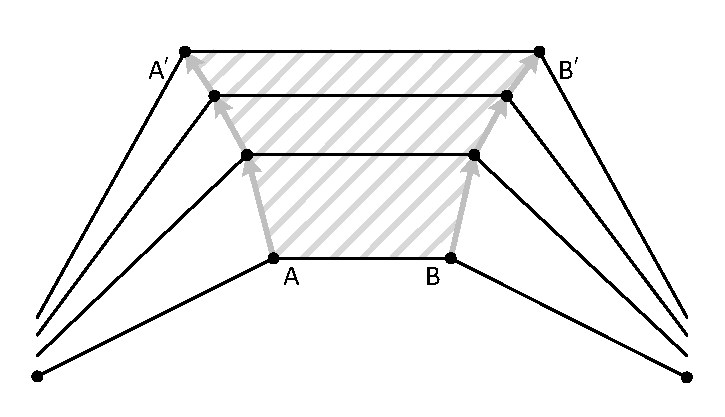
\includegraphics[width=0.48\textwidth]{pics/text_1_remesh_3d/pic_classical_methods_multilayer.pdf}
\captionstyle{center}\caption{Multilayer mesh rebuilding.}\label{fig:pic_classical_methods_multilayer}
\end{figure}

Regardless of the rebuilding method used, a significant increase in accuracy can be achieved using a layered approach \cite{BourgaultCote}.
In this approach, instead of a single rebuilding of the mesh by the volume of accumulated ice in each face ($V(f)$), a fixed number of rebuilding steps $k$ is chosen, and then the procedure is performed $k$ times in a row, but using the volume of ice accumulated in the face $\frac{V(f)}{k}$.
The accuracy increases due to the fact that after each rebuilding step, the normals at the mesh nodes change their direction, and the total volume of the growing ice becomes more curvilinear, takes into account the mesh geometry better, and, as a result, more accurately corresponds to the initial value of $V(f)$ (Fig.~\ref{fig:pic_classical_methods_multilayer}).

\subsubsection{Rebuilding with ice volume conservation}

The articles \cite{Thompson,Tong} describe a stable iterative mesh evolution algorithm that preserves the target volume of ice.
It uses several improvements over the classical methods.

The multilayer approach implemented in this method does not use a constant number of steps -- the value of the increased volume at each step of the algorithm is calculated based on the maximum allowable fraction of the icing time step, after exceeding which numerical instability may occur in the evolution of the surface.
The most obvious case occurs when the face normal projections intersect, in which case too large time step will cause the surface to fold.
In order to  identify faces that will exhibit such behavior at the
current time step, it is assumed that the volume formed by extruding
a triangular face using a parallel displacement plane forms a
prismatoid whose volume is given by the cubic function of the height
$h$:
\begin{equation}\label{Tong:1}
V(h)=ah+bh^2+ch^3.
\end{equation}
where the constants $a$, $b$, $c$ are determined by the  positions
of the face nodes, their normals, and the face normal.
Consider the roots of the quadratic equation, which is obtained as a result of differentiation of the equation (\ref{Tong:1}).
If the roots are positive real values, the smallest positive root determines the height at which the maximum volume is reached, which is denoted as $V_{max}$, otherwise the function is monotonic with increasing and no step restriction is required in this face.
From this, it is possible to calculate the maximum fraction of the icing time step that is required to ensure reasonable volume accumulation behavior.
In addition to this step size limit, a $\alpha_{jiao}$ stability limit has been introduced.
This stability limit is based on how normal directions change as the surface evolves \cite{Jiao}.
Then, the allowable fraction of the time step for the $i$th face is
defined as
\begin{equation*}
\alpha_{\Delta t}^i=
\begin{cases}
\min(s_{\Delta t}\frac{V_{\max}^i}{V_f},\alpha_{jiao},1), \text{if $V_{\max}^i$ exists}, \\
\alpha_{jiao}, \text{if $V_{\max}^i$ doesn't exist},
\end{cases}
\end{equation*}
where $s_{\Delta t}$ ($0 < s_{\Delta t} < 1$) is an  empirically
determined coefficient, $V_f$ is the current remaining ice increment
volume for the $i$th face.
Then, the volume built up for the current step is $\alpha_{\Delta t}
V_f$, where $\alpha_{\Delta t}$ is the global minimum value for all
faces.

Another important feature of the algorithm is the introduction of primary and null spaces, described in \cite{Jiao_null_space_smooth}.
If the evolutionary movement of mesh nodes occurs in primary space, then their movement in zero space will preserve the potential accuracy of the second order of the surface triangulation, so that we can maintain volume when smoothing the mesh surface.
The algorithm uses several types of smoothing.

The first smoothing is the smoothing of the normals in the mesh nodes and faces.
To make smoothing possible in zero space, all normals at nodes are calculated so that they lie in primary space, and the movement of nodes during ice buildup occurs only along their normals.
As evolution progresses, surface noise can increase, and if left unchecked, we can encounter a situation where the dihedral angle between the faces becomes too small and limits the maximum fraction of the icing time step.
To reduce surface noise, local smoothing is applied before ice builds up, adjusting the direction of node displacement in problem areas so that it more closely matches the directions of its neighbors.
This method can improve surface smoothness in some situations.
The main purpose of normal smoothing is to push points out of concave areas where normals can converge locally.
Normal smoothing is achieved using a series of weighted averages,
which are designed to give weight to the normals generated by
problem areas.

\begin{figure}[h]
\centering
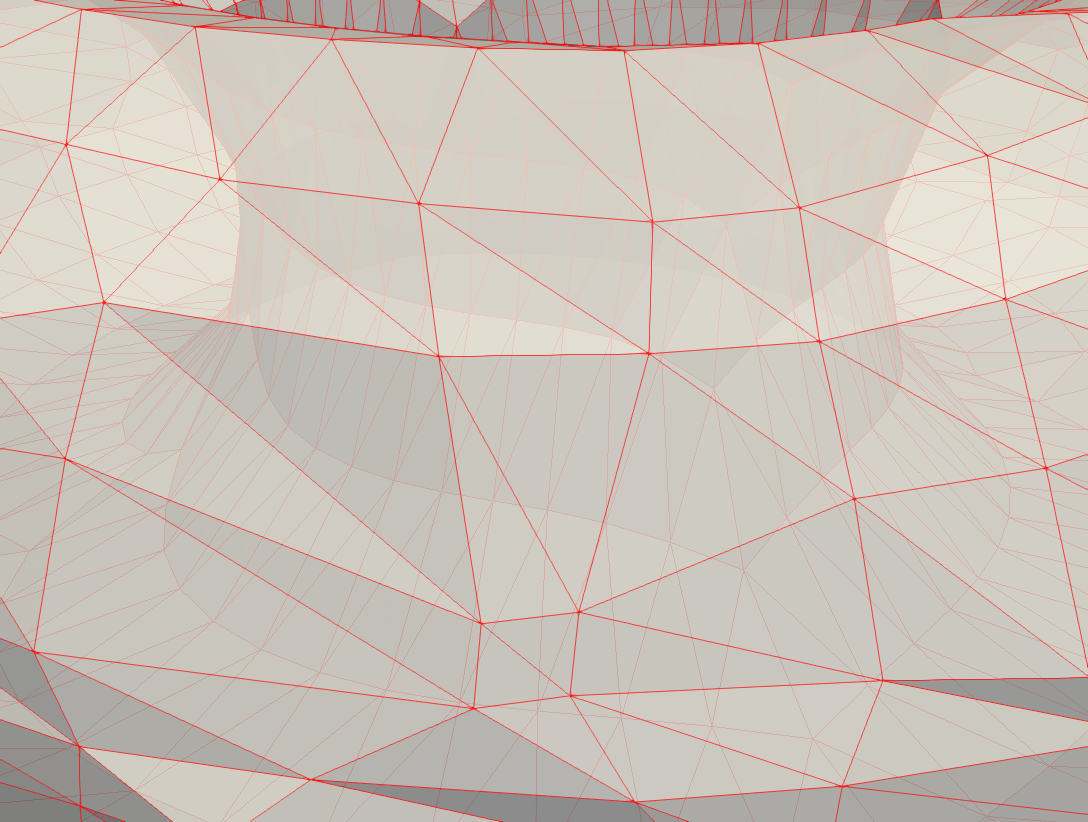
\includegraphics[width=\textwidth]{pics/text_1_remesh_3d/pic_smooth_before.png}
\caption{Mesh before null-space smoothing}\label{fig:pic_smooth_before}
\end{figure}

\begin{figure}[ht]
\centering
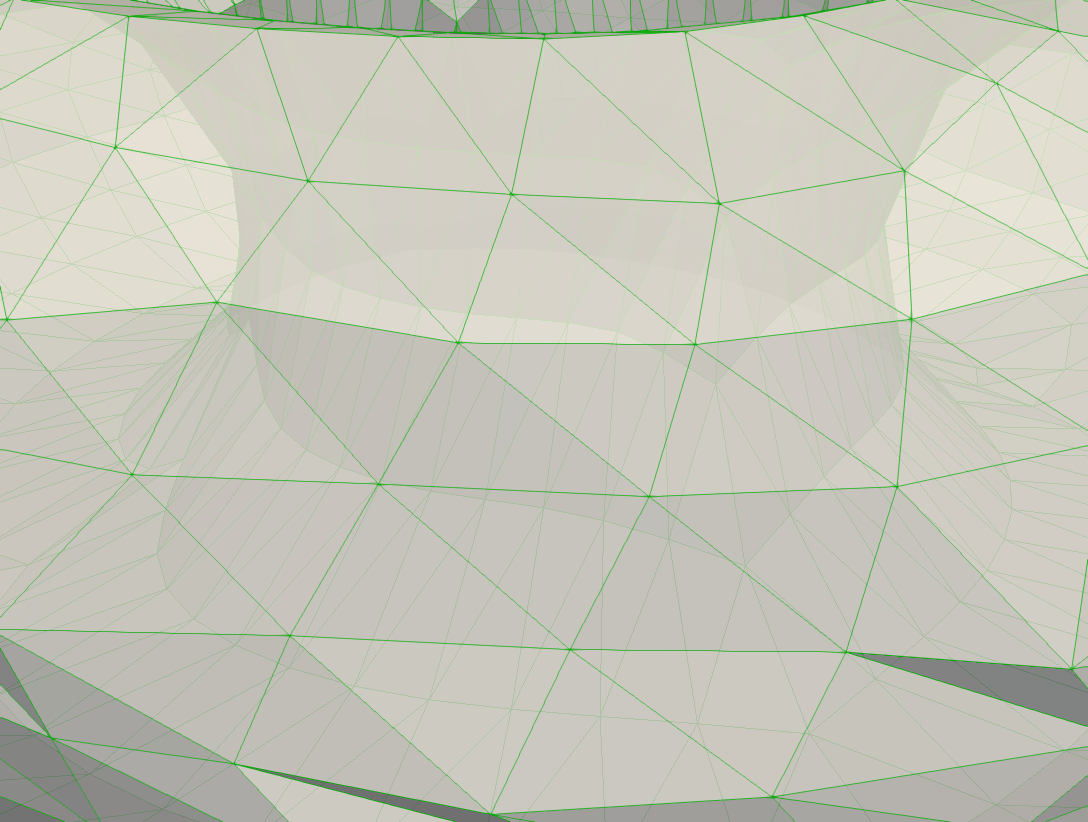
\includegraphics[width=\textwidth]{pics/text_1_remesh_3d/pic_smooth_after.png}
\caption{Mesh after null-space smoothing.}\label{fig:pic_smooth_after}
\end{figure}

The second smoothing is height smoothing.
After calculating the fraction of the time step and the volume that is increased for the current step, it is necessary to determine the height field for the evolution of the surface, which will correspond to this volume, in order to determine the offsets of the mesh nodes from it.
The solution $V(h_i) = \alpha_{\Delta t} V_f$ provides the initial height field that is used to move the surface.
The purpose of the additional height smoothing step is to filter out high-frequency noise in the height field by reducing the difference in height between adjacent faces.
Usually, the heights of two triangular faces that share a common edge will not be equal.
At this step, smoothing of heights is used while preserving the volume by redistributing it between adjacent faces.

The last type of smoothing is null-space smoothing.
Surface evolution will tend to pack nodes into concave regions where surface normals converge, while mesh expansion occurs in convex regions where surface normals diverge.
If the nodes are not reallocated, it may become impossible to continue with a productive and stable time step.
To improve the quality of the surface mesh, the nodes are redistributed on the surface using null-space smoothing.
This method is able to redistribute points while maintaining the integrity of the base geometry.
Null-space is defined by a tangent plane (for smooth areas),  a
tangent line (for surface wrinkles), or empty space (for corners),
nodes moving in it remain on the surface, so that the volume and
shape of the surface can be preserved
(Figs.~\ref{fig:pic_smooth_before} and \ref{fig:pic_smooth_after}).
